
% this file is called up by thesis.tex
% content in this file will be fed into the main document

\chapter{State of the Art} % top level followed by section, subsection


%transition between chapters, usually no more than two parragraphs
The state of the art used in the thesis highlighted the advances in the cloud computing domain and the mobile domain...


% change according to folder and file names
\ifpdf
    \graphicspath{{X/figures/PNG/}{X/figures/PDF/}{X/figures/}}
\else
    \graphicspath{{X/figures/EPS/}{X/figures/}}
\fi

% ----------------------- State of the art ------------------------
%We will try to target 20 -25 word pages for this work
%probably after changing to Latex, the amount of pages will increase but that's because the template
%is double space and half page of each chapter is lost at the beginning, among others.

%XMPP description should fit in one page(text) + a general figure of the federated architecture
%Figures does not count as text
%\section{Jabber and XMPP}
Description of Jabber and XMPP protocol and its usage.


%After the description, try to investigate about how XMPP is utilized in cloud scenarios
%both from academic and commercial points of view, it is unlikely that there is a commercial tool about it, but 
%maybe there is something, you can look for solutions for monitoring smart environments or so
%try to target 2 pages max(text). One or two paragraphs describing each solution
%\section{XMPP to Cloud}
%Some academic related work that can be mentioned is described below
%try to look for them in Google scholar
%From Instant Messaging to Cloud computing, a XMPP review (paper)
%XMPP for cloud computing in bioinformatics supporting discovery and invocation of asynchronous web services
%Performance Evaluation of XMPP on the Web


%arduino along with its component should be one and half page(text) + some images
%if there are configuration we will put them in the appendix
%or we can put a footnote with a link to your github account
\section{Arduino}

Arduino \cite{arduinoHome} is an open-source electronics prototyping platform based on a simple microcontroller board and a development environment for writing software for the board. It is intended for anyone interested in creating interactive solutions. Arduino can take inputs from a variety of sensors and control various actuators and lights. The microcontroller is programmed using the Arduino programming language (based on Wiring) and the Arduino development environment (based on Processing). Arduino IDE enables to choose between different board models, microcontroller programmers and communication ports. 

\todo{add an image of the IDE here... }
Programs (called sketches) are written and uploaded to the board using the Arduino IDE. Each sketch must have two functions- $setup()$ and $loop()$. $setup()$ is the first function called after Arduino is started or rebooted. It is called once and afterwards the function $loop()$ is called consecutively until the board is stopped, restarted or crashes. When a crash occurs, the program is restarted, which means calling $setup()$ again. 

Since programs are written in C/C++, there are a lot of libraries available for use. 

\subsection{Arduino Mega ADK}

Arduino Mega ADK \cite{megaAdk} is one of the most capable boards available. 
The Arduino ADK is a microcontroller board based on the ATmega2560. Similar to the Mega 2560 and Uno, it features an ATmega8U2 programmed as a USB-to-serial converter. It has a USB host interface to connect with Android based phones, 54 digital input/output pins, 16 analog inputs, 4 UARTs (hardware serial ports), a 16 MHz crystal oscillator, USB B, micro B connections and a 2.1mm center-positive power jack. The ADK is designed to be compatible with most shields designed for the Uno, Diecimila or Duemilanove

The ADK has 256 KB of flash memory for storing code (of which 8 KB is used for the bootloader), 8 KB of SRAM and 4 KB of EEPROM (which can be read and written with the EEPROM library).

The Arduino ADK can be powered via the USB connection or with an external power supply. The power source is selected automatically. External (non-USB) power can come either from an AC-to-DC adapter or battery. The board can operate on an external supply of 5.5 to 16 volts. The recommended range is 7 to 12 volts.

\todo{format the text a bit, remove describe what is EEPROM, add an image}

\subsection{Wireless SD Shield}

The Wireless SD shield \cite{arduino_wireless} allows an Arduino board to communicate using a wireless module. The module can communicate up to 100 feet indoors or up to 300 feet outdoors. 

The shield has an on-board switch which allows to select between USB and Micro modes. In USB mode, the shield bypasses Arduino board's microcontroller and communicates directly to the USB-to-serial converter. In Micro mode, data sent from the microcontroller will be transmitted to the computer via USB as well as being sent wirelessly by the wireless module. The microcontroller will not be programmable via USB in Micro mode.

\subsection{RN-XV WiFly Module}

The RN-XV module \cite{rn_xv_module} by Roving Networks is a certified Wi-Fi solution especially designed for customer who want to migrate their existing 802.15.4 architecture to a standard TCP/IP based platform without having to redesign their existing hardware. In other words, if your project is set up for XBee and you want to move it to a standard WiFi network, you can drop this in the same socket without any other new hardware.

The RN-XV module is based upon Roving Networks' robust RN-171 Wi-Fi module and incorporates 802.11 b/g radio, 32 bit processor, TCP/IP stack, real-time clock, crypto accelerator, power management unit and analog sensor interface.The module is pre-loaded with Roving firmware to simplify integration and minimize development time of your application. In the simplest configuration, the hardware only requires four connections (PWR, TX, RX and GND) to create a wireless data connection.

\todo{Add an image of the wireless shield and rn-xv wifi module}	

\subsection{TinkerKit}

TinkerKit \cite{tinkerkit_introduction} is a tool used to build interactive products using Arduino boards. It consists of modules (sensors, actuators) and a sensor shield. The tool greatly simplifies product assembly, because instead of building circuits out of low level components, all the modules can be attached to the TinkerKit sensor shield with a snapping cable.

Here is the mega sensor shield used in this project...
\todo{Add a figure of the mega sensor shield}

The modules are divided into sensors and actuators. Sensors can measure their surrounding environment (provide input) and actuators perform actions (provide output). The sensors used are thermistor, LDR and Hall. 

Thermistor sensor \cite{thermistor_sensor} is a resistor whose resistance changes significantly with temperature. The module's output ranges from 0V to 5V

Hall sensor \cite{hall_sensor} creates a voltage related to the magnetic field near the sensor. It can detect the presence of a nearby magnet or magnetic field induced in a coil or wire. The output ranges from 0V (no presence) to 5V (presence detected). 

Light Dependent Resistor or LDR \cite{light_sensor} is a variable resistor whose resistance is decreased when light falls on the sensor. The module's output is 5V when the module receives no light and 0V when bright light falls on it.

%Fuzzy logic is the main contribution, therefore, you can write here up to 5 pages
\section{Fuzzy Logic}

\todo{add citations here...}

Fuzzy logic is a form of logical reasoning which is based on approximate instead of exact reasoning. When traditional reasoning has binary values like true (1) and false (0), fuzzy logic has values ranging from 0 to 1. These values represent a partial truth or in other words the degree of truth. This is similar to probability which also describes partial truth. The difference between probability and fuzzy logic is that whereas fuzzy logic describes how true something is, probability describes how likely it is for something to be true. 

\subsection{Fuzzy Set}
Fuzzy sets are the main building blocks of fuzzy logic. In traditional set theory where an element can either belong or not belong to a set. With fuzzy sets, an element has a degree of membership to a set. 

Fuzzy sets are represented by membership functions, which measure the degree of membership (DOM) a given value has to the set. Membership functions are usually depicted graphically and have names based on the shape of their graphical representation. Membership functions are depicted as 2-dimensional graphs, where the x-axis represents the values and y-axis the degrees of membership (ranges from 0 to 1). The degree of membership for a given value can be found by projecting vertically to the upper boundary of the membership function. 

The most used membership functions are triangular and trapezoidal functions. Sample sets are shown in \autoref{sample_fuzzy_sets}. Based on these graphs the DOM can easily be seen. Furthermore, from this graph can be seen the difference between fuzzy sets and traditional sets. Let us assume that the values represent age, trapezoidal membership function describes young people and triangular describes middle-aged people. Now when we have an age value that is between points $X_2$ and $X_3$, this value belongs to both the young and middle-aged sets. The difference is in the value of DOM to either set. When the value is nearer to point $X_3$ than to $X_2$ the statement that it belongs to the middle-aged set has a higher truth value.  

\begin{figure}[h]
\centering
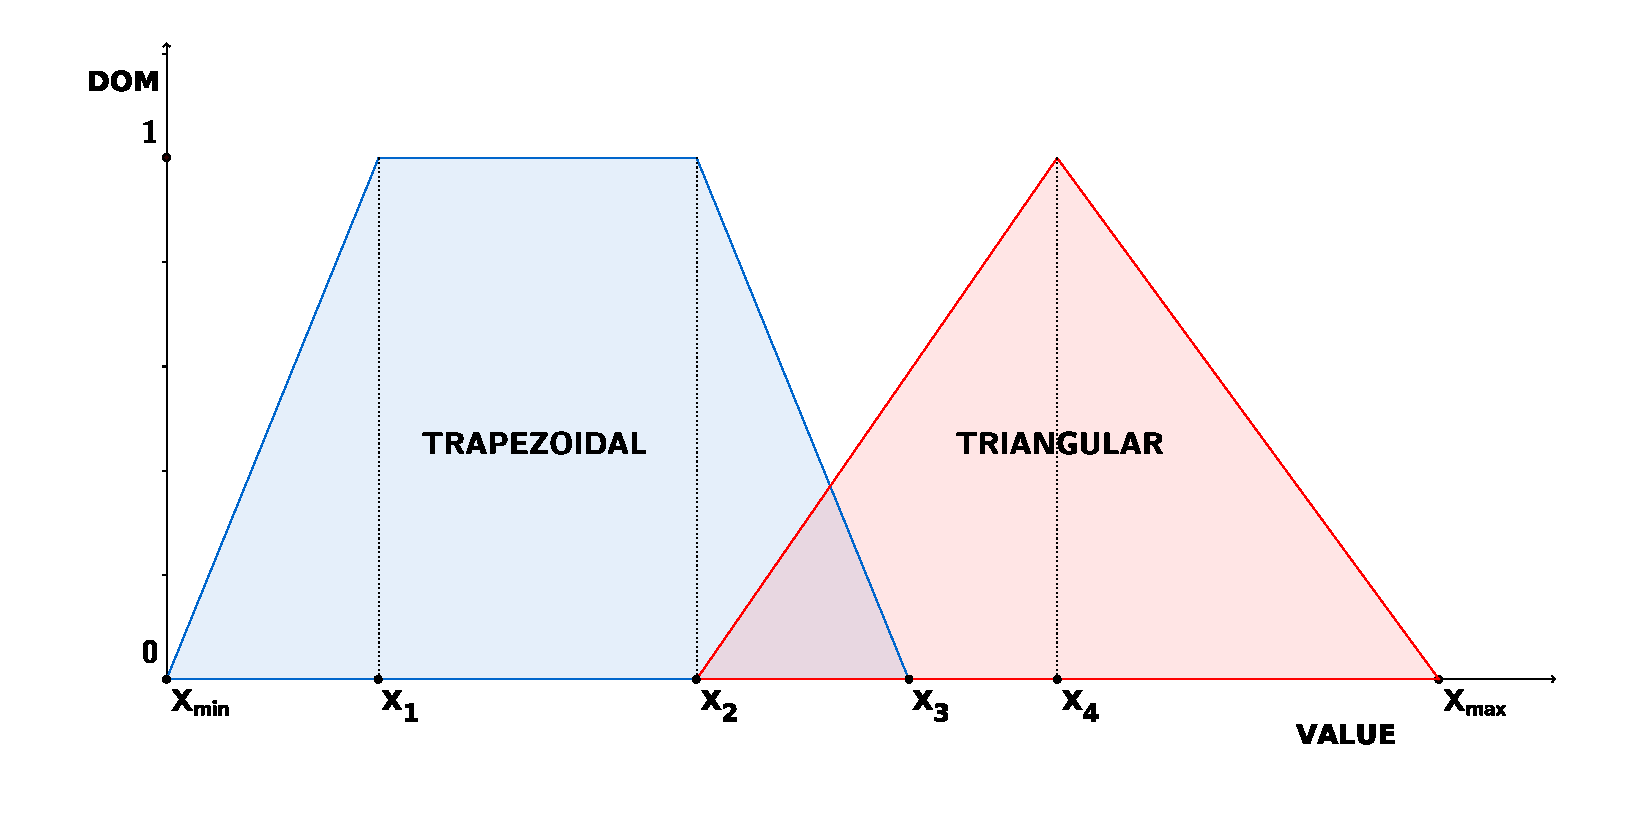
\includegraphics[scale=0.58]{2/figures/sample_sets.pdf}
\caption{Trapezoidal and Triangular Membership Functions}
\label{sample_fuzzy_sets}
\end{figure}

\subsection{Fuzzy Set Operations}

Fuzzy set operations \cite{fuzzy_sets} are a generalized version of standard set operations. The most widely used generalization is referred to as the standard fuzzy set operations. This generalization includes three main operations - complement, union and intersection. Lets assume we have two fuzzy sets with membership functions $A$ and $B$, then these operations can be defined as: 

\begin{tabbing}
\textbf{Complement:}\hspace{1em} \= $\neg A(x) = 1 - A(x)$\\
\textbf{Intersection:}\hspace{1em} \> $(A \cap B)(x) = min\{A(x), B(x)\}$\\
\textbf{Union:}\hspace{1em} \> $(A \cup B)(x) = max\{A(x), B(x)\}$\\
\end{tabbing}

\subsection{Fuzzy Control Systems}

Fuzzy control systems \cite{fuzzy_control_introduction} take a heuristic modeling approach to describing the controllable domain. The heuristic model is based on a set of rules in the for: \textbf{if} $<condition>$ \textbf{then} $<action>$. 

With the fuzzy logic part, the control system has a set of input variables and output variables, which are mapped into fuzzy sets. These variables and fuzzy sets have linguistic variables called labels. 

These fuzzy sets and rules combined gives us a control system which consists of a set of rules where conditions and actions are defined as fuzzy values. For example if we have an input variable $temperature$ with a fuzzy set labelled $cold$ and an output variable $heat$ with a fuzzy set labelled $on$, we could write a following rule: IF $temperature = cold$ THEN $heat = on$. Based on this rule, the system can decide that if the temperature is cold then the heat should be turned on. 

In an actual system there are multiple rules defined. As rules are activated only if their condition holds, the process of adding rules and variables has little computational overhead making the rulebase easily extendable.

Fuzzy control systems are mostly based on experience and experiments rather than actual mathematical modelling. Furthermore, as input and output variables are mapped into fuzzy sets, which have linguistic labels, the systems control rules are easily understandable. This makes fuzzy control systems usable in cases where the actual users have little knowledge of the implementation details. Instead, they can focus on the control process by defining understandable variables, their fuzzy sets and rules based on these sets. 
%This one is not necessary, since we will just mention the tool and it will be cited in chapter 4
%\section{Power supply}
%Overview of the PeakTech 1890 power supply.

\subsubsection{Fuzzy control process}

The decision making process has 4 main steps - fuzzification, rule evaluation, interference and defuzzification. These steps assume that the rules, input and output variables have already been defined.  of the model

The first step in the process is fuzzification. In this step, the system's input and/or output variables are mapped into fuzzy sets. Each input variable can have one or more associated fuzzy sets. What this process does is decompose the crisp input values into fuzzy values. These fuzzy values are expressed by linguistic terms (labels) which can then be used in the rule evaluation process.

The next step is to use the fuzzified values in rule evaluation. A set of predefined rules is evaluated based on the fuzzy values created during the fuzzification process. Rules are activated when their condition holds, otherwise they are skipped. After all rules have been considered, the activated ones are gathered together. The results or actions of these rules are the basis of the next step called defuzzification.

Defuzzification is the final step in the fuzzy control process. This part is responsible for translating the fuzzy values (linguistic terms) into a crisp quantifiable result. Usually in the previous step, rule outputs will be linguistic terms (fuzzy sets) and corresponding degrees of membership for a defined output variable. In the defuzzification part, the different fuzzy sets and their DOMS for the output variable must be added together somehow to produce a final output. 

There are several defuzzification methods. The simplest of which would be to use the fuzzy set with the highest DOM as the final result. However, center of gravity is the most commonly used method. First, the different degrees of membership calculated from rules must be combined for each output variable's fuzzy sets. Then, the membership functions are depicted of a graph and for each fuzzy set, the top of the membership function is cut of in a straight horizontal line at the height of the DOM value. When this is done for all fuzzy sets of the output variable, the center of gravity for the remaining shape is calculated. The center point's projection on the value axis (usually the x-axis) is the crisp result.

\section{Simple Linear Regression}

\todo{Add simple linear regression here, too?}

%add figures
%\begin{figure}
%\centering
%\includegraphics[width=0.65\textwidth]{2/figures/Cloud/funambolArchitecture.png}
%\caption{Funambol architecture}
%\label{fig:funambolArchitecture}
%\end{figure}


% ---------------------------------------------------------------------------
% ----------------------- end of thesis sub-document ------------------------
% --------------------------------------------------------------------------- 
